\chapter{Qualitätssicherung}
\label{chap:Qualitätssicherung}

Nach der erfolgreichen Implementierung des Source-To-Source Compilers soll mithilfe einer Xamarin.Forms App überprüft werden,  ob der Compiler so arbeitet wie zu erwarten ist.  

\section{Testobjekt}
Die App wurde mit der aktuellen Version 5.0.0.2012 des Xamarin.Forms Frameworks realisiert und verwendet die Erweiterungen Xamarin. Essentials.  Die Anwendung wurde mit dem Ziel entworfen möglichst viele Funktionalitäten von Xamarin.Forms abzubilden,  sie hat jedoch nicht den Anspruch einer vollständigen Testabdeckung.  Die App verzichtet, bis auf die Metadaten und Ressourcen weitestgehend auf plattformspezifische Implementationen. Im folgenden werden die Funktionalitäten und Eigenschaften der mobilen Anwendung erläutert und mit Hilfe von iOS Screenshots visualisiert,  die entsprechenden Android Screenshots werden der Vollständigkeitsannahme in \hyperref[chap:AnhangAndroidScreenshots]{Anhang IV} dargestellt.

Der Name und das Anwendungsicon sind wichtige Merkmale anhand welcher Anwender die App identifizieren können.  Nach dem Start der Anwendung wird eine  Menüstruktur angezeigt,  über den verschiedene Bereiche der Anwendung angesteuert werden können.  Das Menü dient als zentraler Startpunkt der Anwendung und somit als Wurzel für die Navigation durch die App.  Abbildung \ref{fig:TestObjectI} zeigt sowohl das Icon und den Namen der App auf dem iOS Homescreen,  das Menu der App und eine Seite für die Visualisierung der verfügbaren Steuerelemente.
\newpage
\begin{figure}[!ht]
 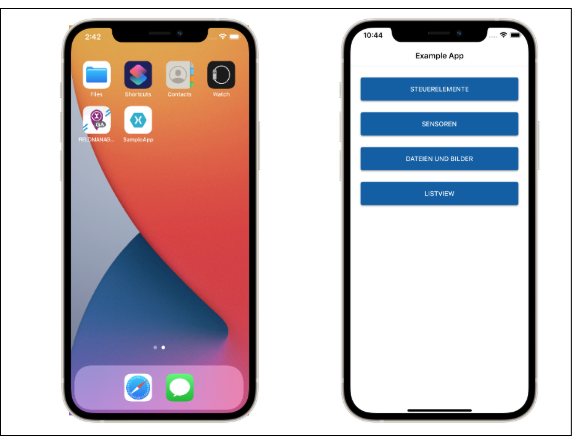
\includegraphics[width=\textwidth,keepaspectratio]{Images/Screenshot/AppIconAndMenu.png}
 \caption{Test Objekt Screenshots I}
 \label{fig:TestObjectI}
\end{figure}

Über das Menü kann neben den Steuerelementen auch zu einer Ansicht navigiert werden,  die die Werte der Smartphone Sensoren ausgibt.  Dazu gehören der Beschleunigungssensor,  der Kompass,  das Gyroscope und das Magnetomet. Außerdem können Bilder über die Kamera aufgenommen oder aus der Galerie ausgewählt werden.  Diese Ansichten werden in Abbildung \ref{fig:TestObjectII} dargestellt.

\begin{figure}[!ht]
 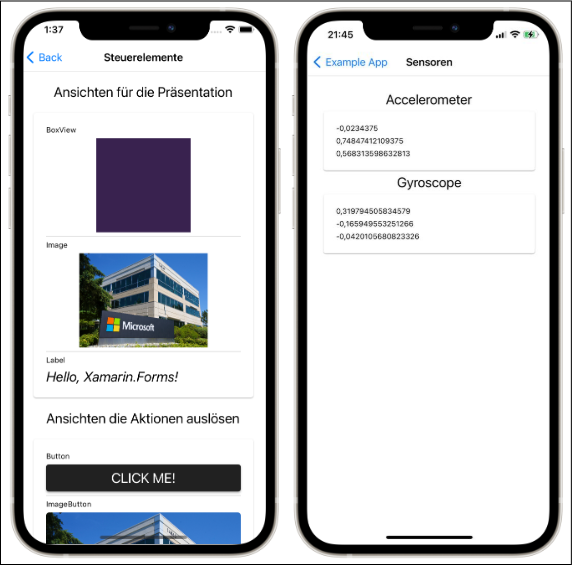
\includegraphics[width=\textwidth,keepaspectratio]{Images/Screenshot/Sensors.png}
 \caption{Test Objekt Screenshots II}
 \label{fig:TestObjectII}
\end{figure}


\section{Testfälle}
Um den Compiler zu Testen ist es notwendig Testfälle zu definieren und zu überprüfen, ob der Compiler die Xamarin.Forms App so übersetzt, wie es zu erwarten .   Zu diesem Zweck werden in diesem Abschnitt Testfälle definiert die sich aus den ermittelten Unterschieden zwischen beiden Frameworks,  sowie der Programmiersprachen ergeben.  Tabelle \ref{tab:Testapp} zeigt die Testfälle für die Metadaten der mobilen Anwendung. 

\begin{table}[!ht]
\begin{tabularx}{\textwidth}{l|l|X}
   \textbf{ID} & \textbf{Komponente} & \textbf{Beschreibung} \\
\hline
1             & App-Icon           	& Prüfen ob das App-Icon übernommen wurde                      			 \\ 
2             & App-Name          	& Prüfen ob das App-Name übernommen wurde                      		 \\ 
3             & SDK Versionen      & Prüfen ob die SDK Versionen übernommen wurden                      \\ 
4             & Seitenname           				& In der Navigationsleiste wird der Name der aktuellen Seite angezeigt                      			 \\ 
5          	  & Navigation         			  	& Mit Hilfe des Menüs kann navigiert werden                      			 \\ 
6             & Zurück Navigation           	& Über die Navigationsleiste kann zurrück Navigiert werden                      			 \\ 
7             & Gyroscope auswerten           	& Die Werte werden in der App angezeigt.                      			 \\ 
8             & Accelerometer auswerten           	& Die Werte werden in der App angezeigt.                   			 \\ 
9             & Compass auswerten           	& Die Werte werden in der App angezeigt.                			 \\ 
10            & Magnetometer auswerten           	& Die Werte werden in der App angezeigt.                			 \\ 
11            & Sensor nicht verfügbar           	& Wenn ein Sensor nicht verfügbar ist, wird ein Fehler angezeigt          			 \\ 
12            & Steuerelemente wurden ausgetauscht           	& Alle Steuerelemente werden angezeigt        			 \\ 
13            & Ereignisse funktionieren           	&  Steuerelemente reagieren wie gewohnt     			 \\ 
14            & Bild aus Ressourcen laden           	& Ein Bild aus den Ressourcen wird in der App angezeigt                      			 \\ 
15             & Bild aus dem Web laden           	& Ein Bild aus dem Internet wird in der App                      			 \\ 
\end{tabularx}
\caption{Testfälle der Test App}
 \label{tab:Testapp}
\end{table}



\section{Testablauf}
Für den Start des Testlaufes wird die grafische Benutzeroberfläche gestartet. Anschließend wird das entwickelte Testobjekt als Xamarin.Forms Projekt und ein leerer als Ordner als Zielverzeichnis ausgewählt. Anschließend kann die Übersetzung gestartet werden.  Aufgrund der vielen Dateizugriffe und durchzuführenden Aktivitäten kann die Übersetzung der Anwendung eine gewisse Zeit in Anspruch nehmen. 
Nach dem erfolgreichen Durchlauf der Übersetzung werden im Front-End die Informationen bezüglich der Übersetzung ausgegeben.  
Anschließend kann mit Hilfe von Visual Studio Code die übersetzte Flutter Anwendung gestartet werden.  In einem ersten Schritt können die Metadaten von sowohl Android als auch iOS App mit denen der Xamarin.Forms App verglichen werden, um zu validieren ob diese entsprechend übernommen wurden.
Nach einer erfolgreichen Überprüfung können nun die einzelnen Ansichten der Flutter App überprüft werden.  Dafür werden im folgenden die Screenshots der Flutter App dargestellt.  Dabei werden wie in der Einführung des Testobjektes die selben Bilder in der selben Reihenfolge dargestellt.  Die entsprechenden Screenshots von Android befinden sich ebenfalls im Anhang dieser Arbeit. 

\section{Testauswertung}
Dieser Test zeigt,  dass das Testobjekt vollständig überführt wurde.  Das Testobjekt kann jedoch nicht alle Xamarin.Forns Funktionalitäten abbilden und demonstriert ausschließlich die Funktionsfähigkeit des Prototypens.  